\documentclass[12pt,xcolor=dvipsnames]{beamer}

% Pakete
\usepackage[utf8]{inputenc}
\usepackage[german]{babel}

% AMS Pakete
\usepackage{amsmath}
\usepackage{amsfonts}
\usepackage{amssymb}

\usepackage{braket}

\usepackage{multirow}

% Einheiten
\usepackage{siunitx}
\sisetup{
	output-decimal-marker={,},
	separate-uncertainty
}

% Grafiken
\usepackage{graphicx}
\usepackage{tabularx}
\newcommand{\korr}[1]{{\textcolor{Yellow}{(#1)}}}

% Theme
\usetheme{Boadilla}
\usecolortheme{rose}
\useoutertheme{infolines}
\useinnertheme{rectangles}
\setbeamertemplate{itemize subitem}[triangle]

\usefonttheme[onlymath]{serif}

% [num] Zitationen
\setbeamertemplate{bibliography item}[text]

% Navigationsleiste ausschalten
\beamertemplatenavigationsymbolsempty

\DeclareMathOperator{\divergence}{div}

\author[Christopher Deutsch]
{Christopher Deutsch}

\title
{Atomfallen}

\subtitle
{Ein Überblick der wichtigsten Fallen}
%\logo{}

\institute[]
{Rheinische Friedrich-Wilhelms-Universität Bonn \\
Proseminar Präsentationstechnik SS15}

\date{8. Juni 2015}

%\setbeamercovered{transparent}
%\setbeamertemplate{navigation symbols}{}

\begin{document}
\maketitle

\begin{frame}{Inhalt}
	\tableofcontents
\end{frame}


\section{Motivation}

\begin{frame}{Was sind Atomfallen?}
	\begin{itemize}
		\item Einschluss von Atomen im Raumvolumen durch ortsabhängige Kräfte
		
		\item Fangen ohne materielle Wände wünschenswert:
		\begin{itemize}
			\item minimaler Einfluss auf die innere Struktur des Ensembles
			
			\item thermische Isolation von der Umgebung
		\end{itemize}

	\end{itemize}
\end{frame}

\begin{frame}{Grundlagen}
	\begin{itemize}
		\item Einschluss der Atome durch Potentialtopf:
			\begin{figure}
				\centering
				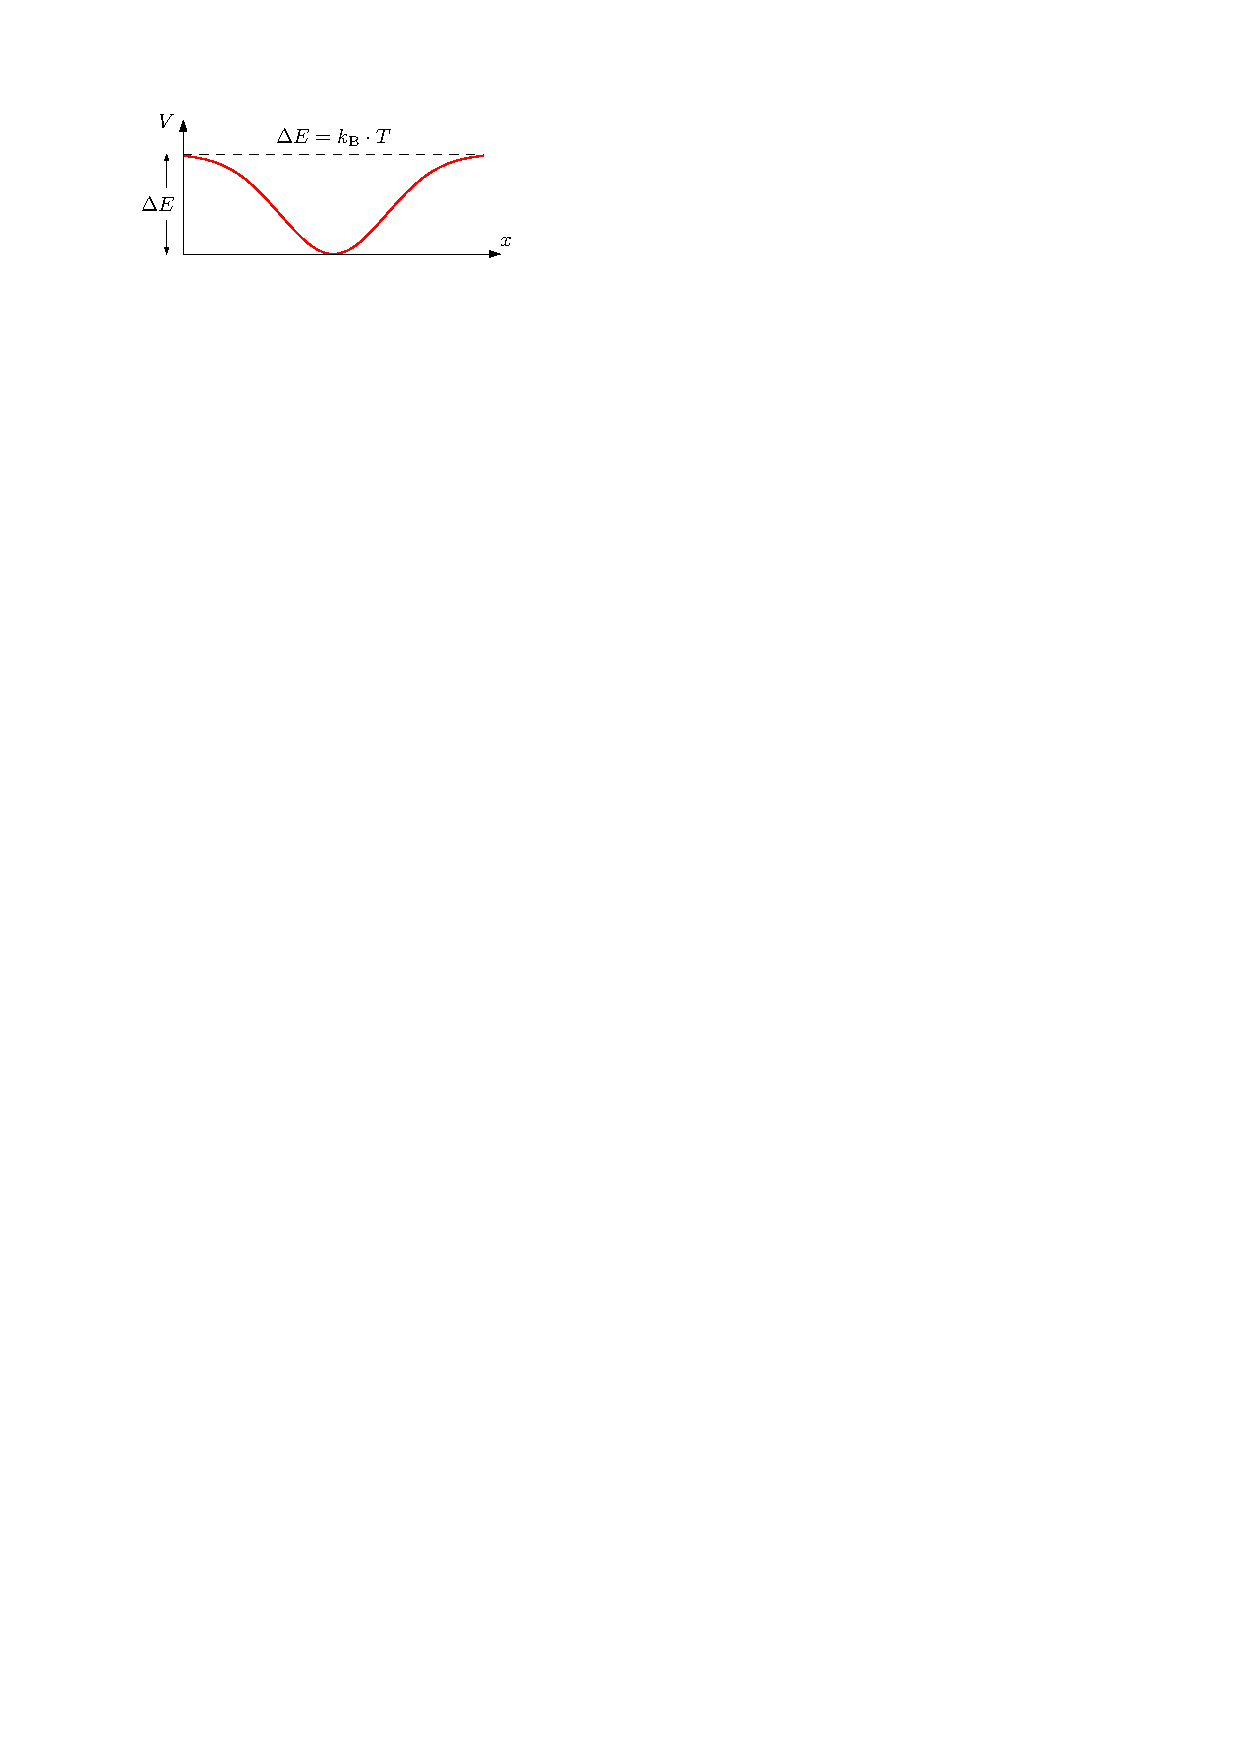
\includegraphics[width=0.6\textwidth]{./figures/fallentiefe.pdf}
			\end{figure}
		\item Energie wird charakterisiert durch Temperatur:
		\begin{align*}
		E = k_\mathrm{B} \cdot T
		\end{align*}
		
		\item Kühlung und Atomfallen stehen in ständiger \korr{Korrelation}
		
	\end{itemize}

\end{frame}

\begin{frame}{Wofür braucht man Atomfallen?}
	\begin{itemize}
		\item Strukturuntersuchung von Materie bei niedrigen Temperaturen (BEC, Ionenkristalle)
		
		\item hochauflösende Spektroskopie
			\begin{itemize}
				\item Minimierung von Dopplereffekt und Zeitdilatation
				\item Frequenzstandards / Atomuhren (NP 1989 Ramsey, Paul, Dehmelt)
			\end{itemize}
		
		\item Manipulation von quantenmechanischen Systemen einzelner Teilchen (Qubit)
	\end{itemize}
\end{frame}


\section{Paul-Falle}

\begin{frame}{Grundlagen der Ionenfallen}
	\begin{itemize}
		\item Ausnutzung der Kraft auf geladene Teilchen im elektromagnetischen Feld
			\begin{itemize}
				\item Kraft auf freie Ladungsträger ist groß (vgl. mit Dipol/Streukraft) ($10^6 \si{K}$)
			\end{itemize}
		
		\item \alert{Problem:} Maxwell-Gleichungen verbieten Fangen von geladenen Teilchen durch elektrostatische Felder (Earnshaw-Theorem)
		
		\vspace{0.5cm}
		\centering
		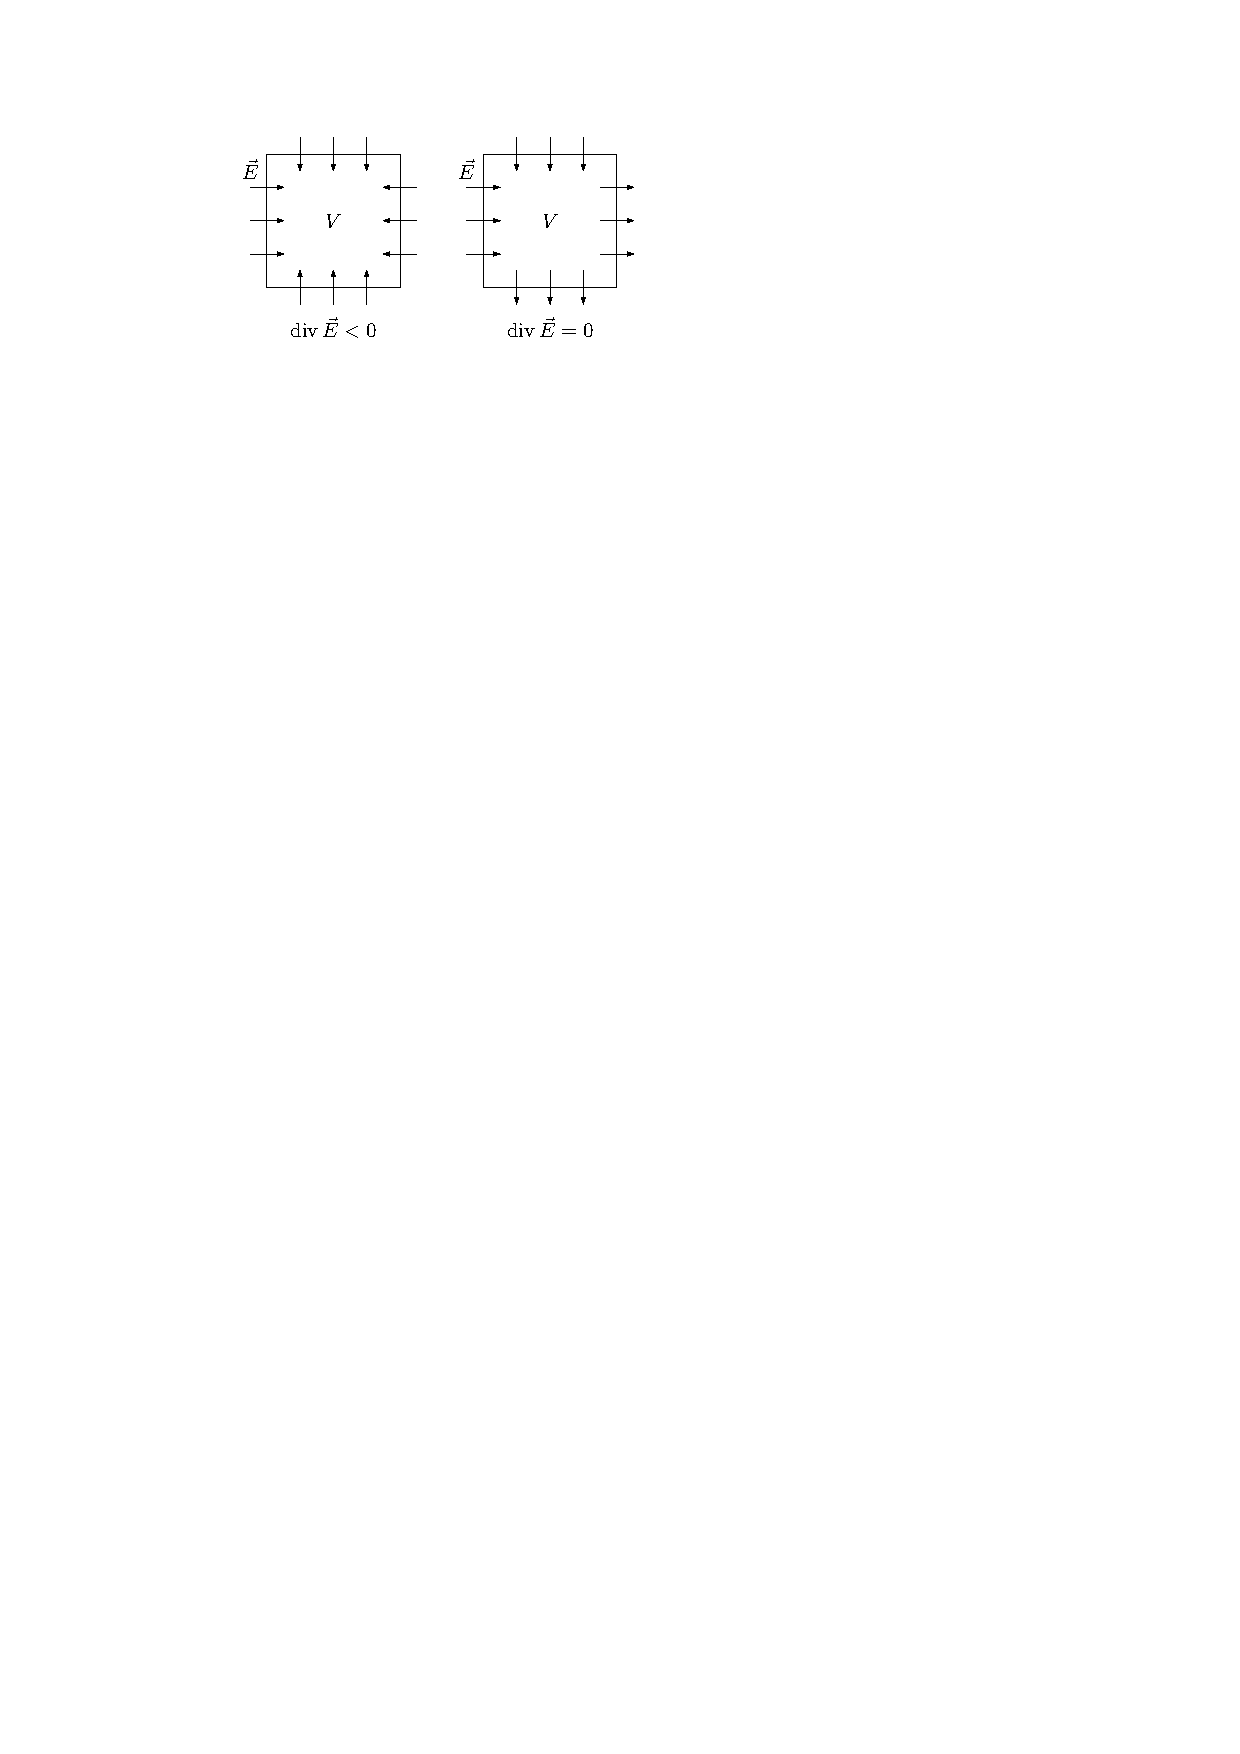
\includegraphics[width=0.55\textwidth]{./figures/earnshaw.pdf}
		
	\end{itemize}
\end{frame}


\begin{frame}{Lineare Paul-Falle ($x$-$y$-Ebene)}
	\begin{itemize}
		\item Ausnutzung der Trägheit des Ions im Quadrupol-Wechselfeld
		\begin{itemize}
			\item Basierend auf dem Prinzip der starken Fokussierung der Beschleunigerphysik (1952 Paul Planung \SI{500}{MeV}-Synchrotron)
		\end{itemize}
	\end{itemize}
	
	
	\begin{minipage}[t]{0.5\textwidth}
		\centering
		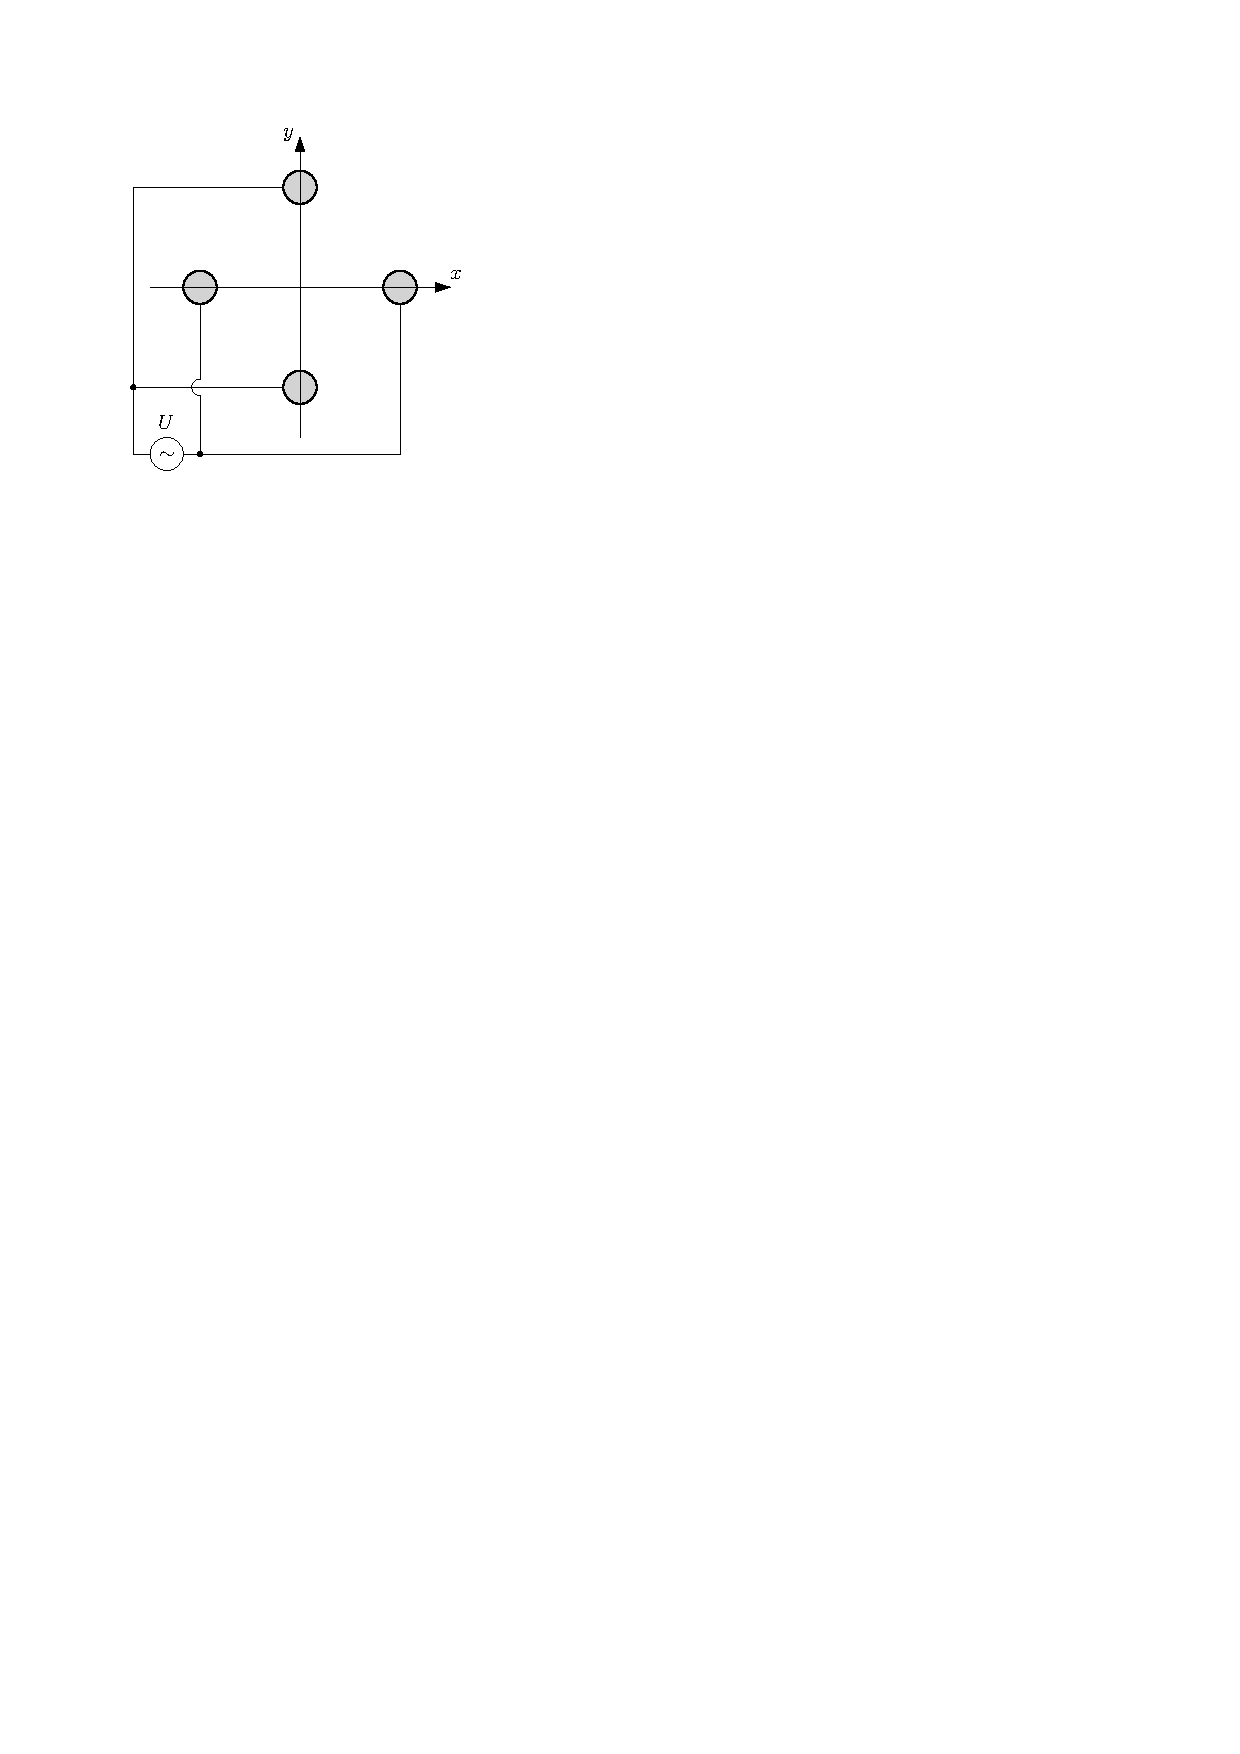
\includegraphics[width=0.8\textwidth]{./figures/lineare_paulfalle_xy.pdf}
	\end{minipage}%
	\begin{minipage}[t]{0.5\textwidth}
		\centering
		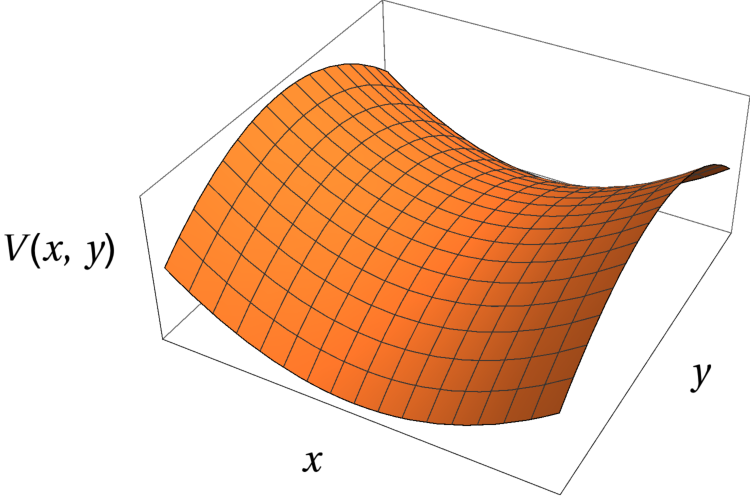
\includegraphics[width=0.95\textwidth]{./figures/sattelpotential.pdf}
	\end{minipage}
\end{frame}

%\begin{frame}{Lineare Paul-Falle ($x$-$y$-Ebene)}
%	\begin{columns}[t]
%		\column{0.5\textwidth}
%		Quadrupol:
%		\begin{figure}[h]
%			\centering
%			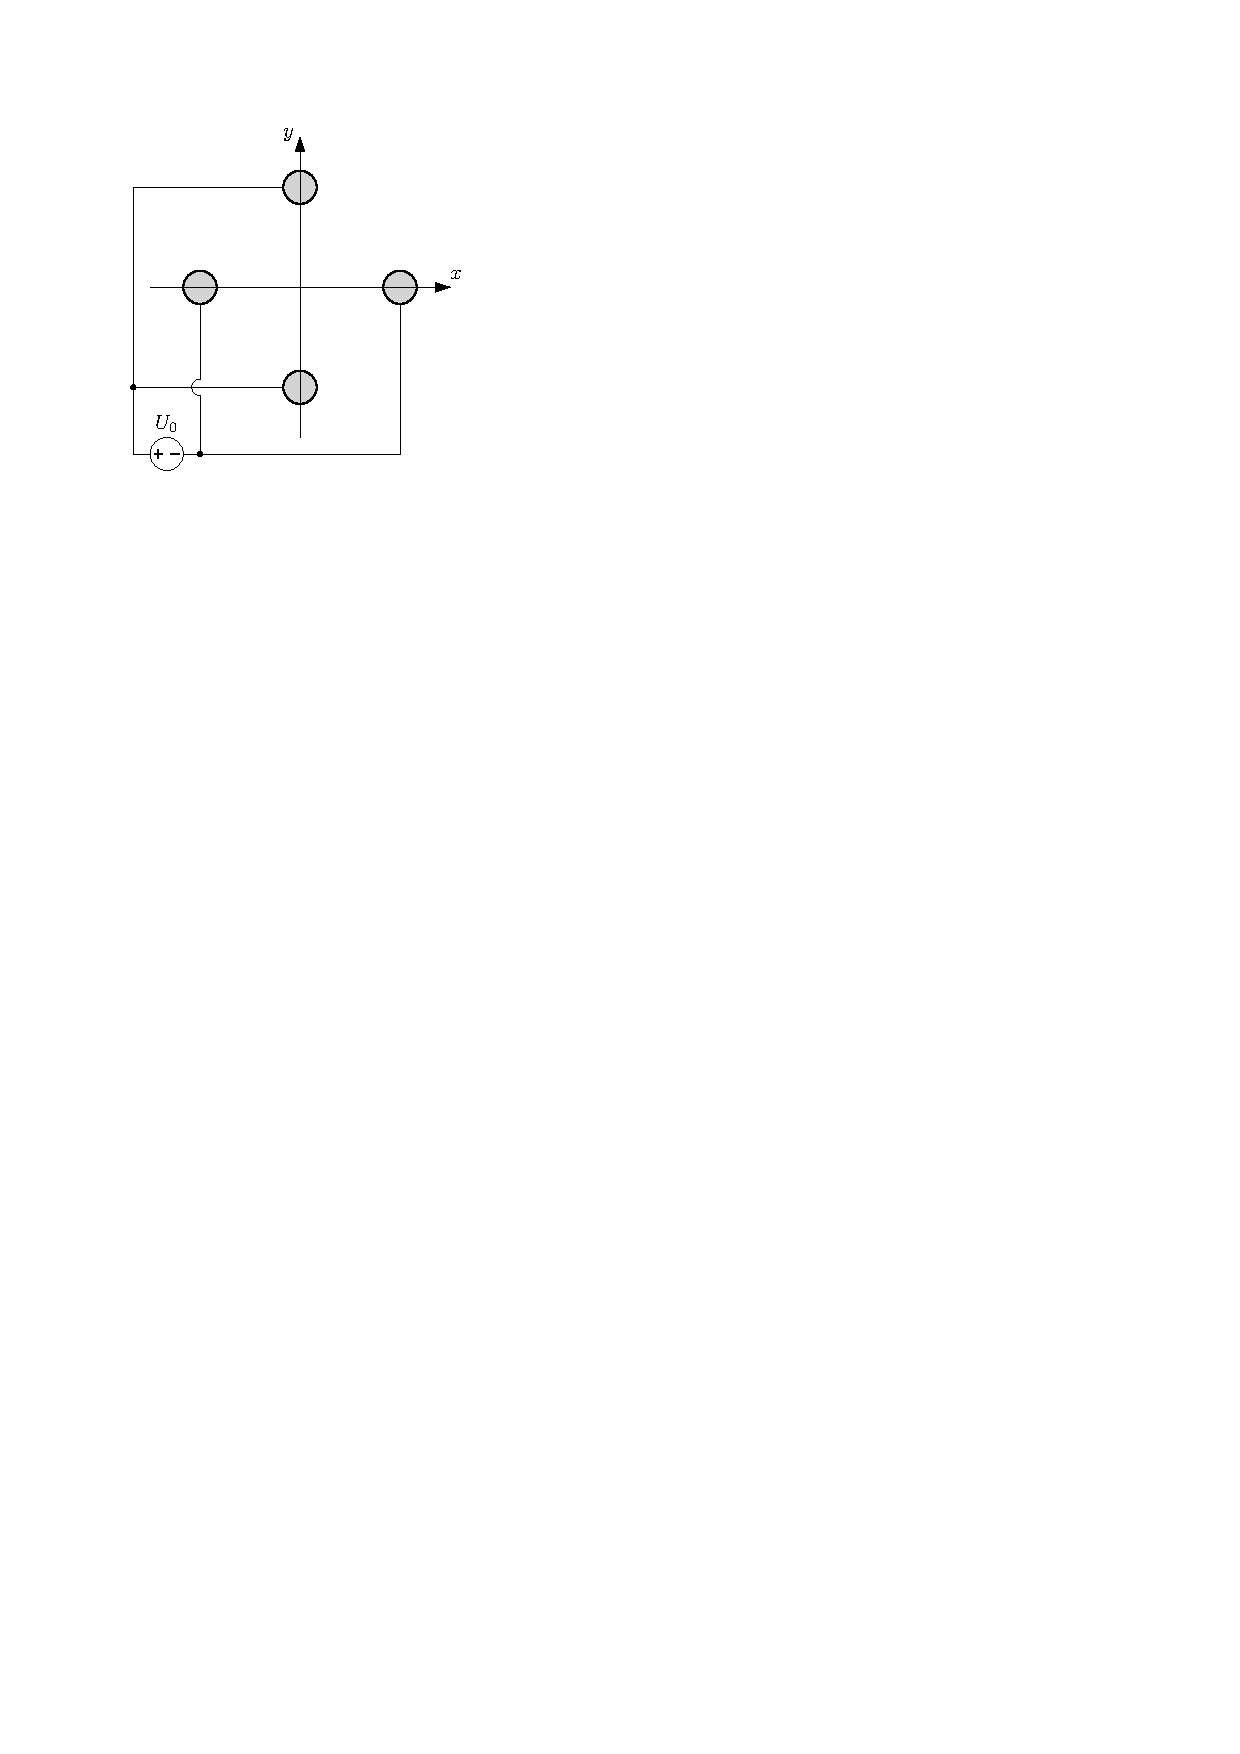
\includegraphics[width=0.8\textwidth]{./figures/lineare_paulfalle_xy_statisch_swapped.pdf}
%		\end{figure}
%		
%		\column{0.5\textwidth}
%		Quadrupol-Potential:
%		\begin{align}
%		\phi = \phi_0 - \frac{U_0}{2 \, r_0^2} (x^2-y^2)
%		\end{align}
%		\begin{figure}[h]
%			\centering
%			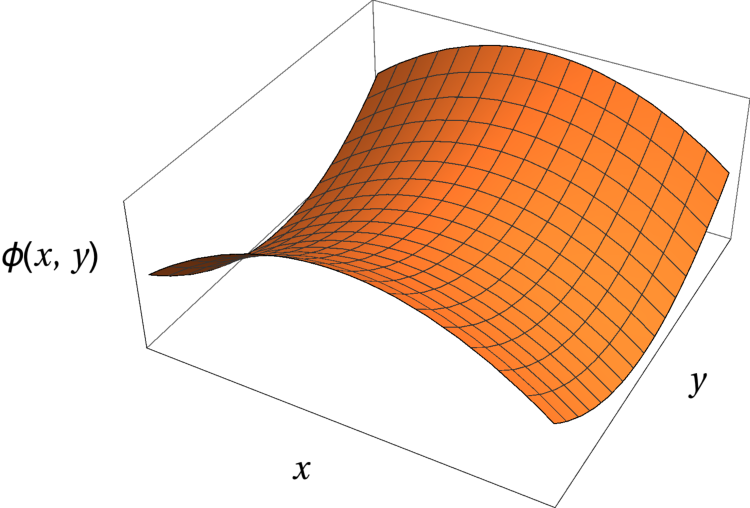
\includegraphics[width=0.95\textwidth]{./figures/sattelpotential2.pdf}
%		\end{figure}
%	\end{columns}
%\end{frame}

\begin{frame}{Lineare Paul-Falle (Erweiterung auf die $z$-Achse)}
	\begin{columns}[t]
		\column{0.5\textwidth}
		\begin{itemize}
				\item dreidimensionales Fangen durch Endkappenelektroden
				
				\item Stabilität abhängig von Feld- und Teilcheneigenschaften
				\begin{itemize}
					\item Massenspektrometrie möglich
				\end{itemize}
		\end{itemize}
		
		\column{0.4\textwidth}
			\vspace{-0.4cm}
			\begin{figure}[h]
				\centering
				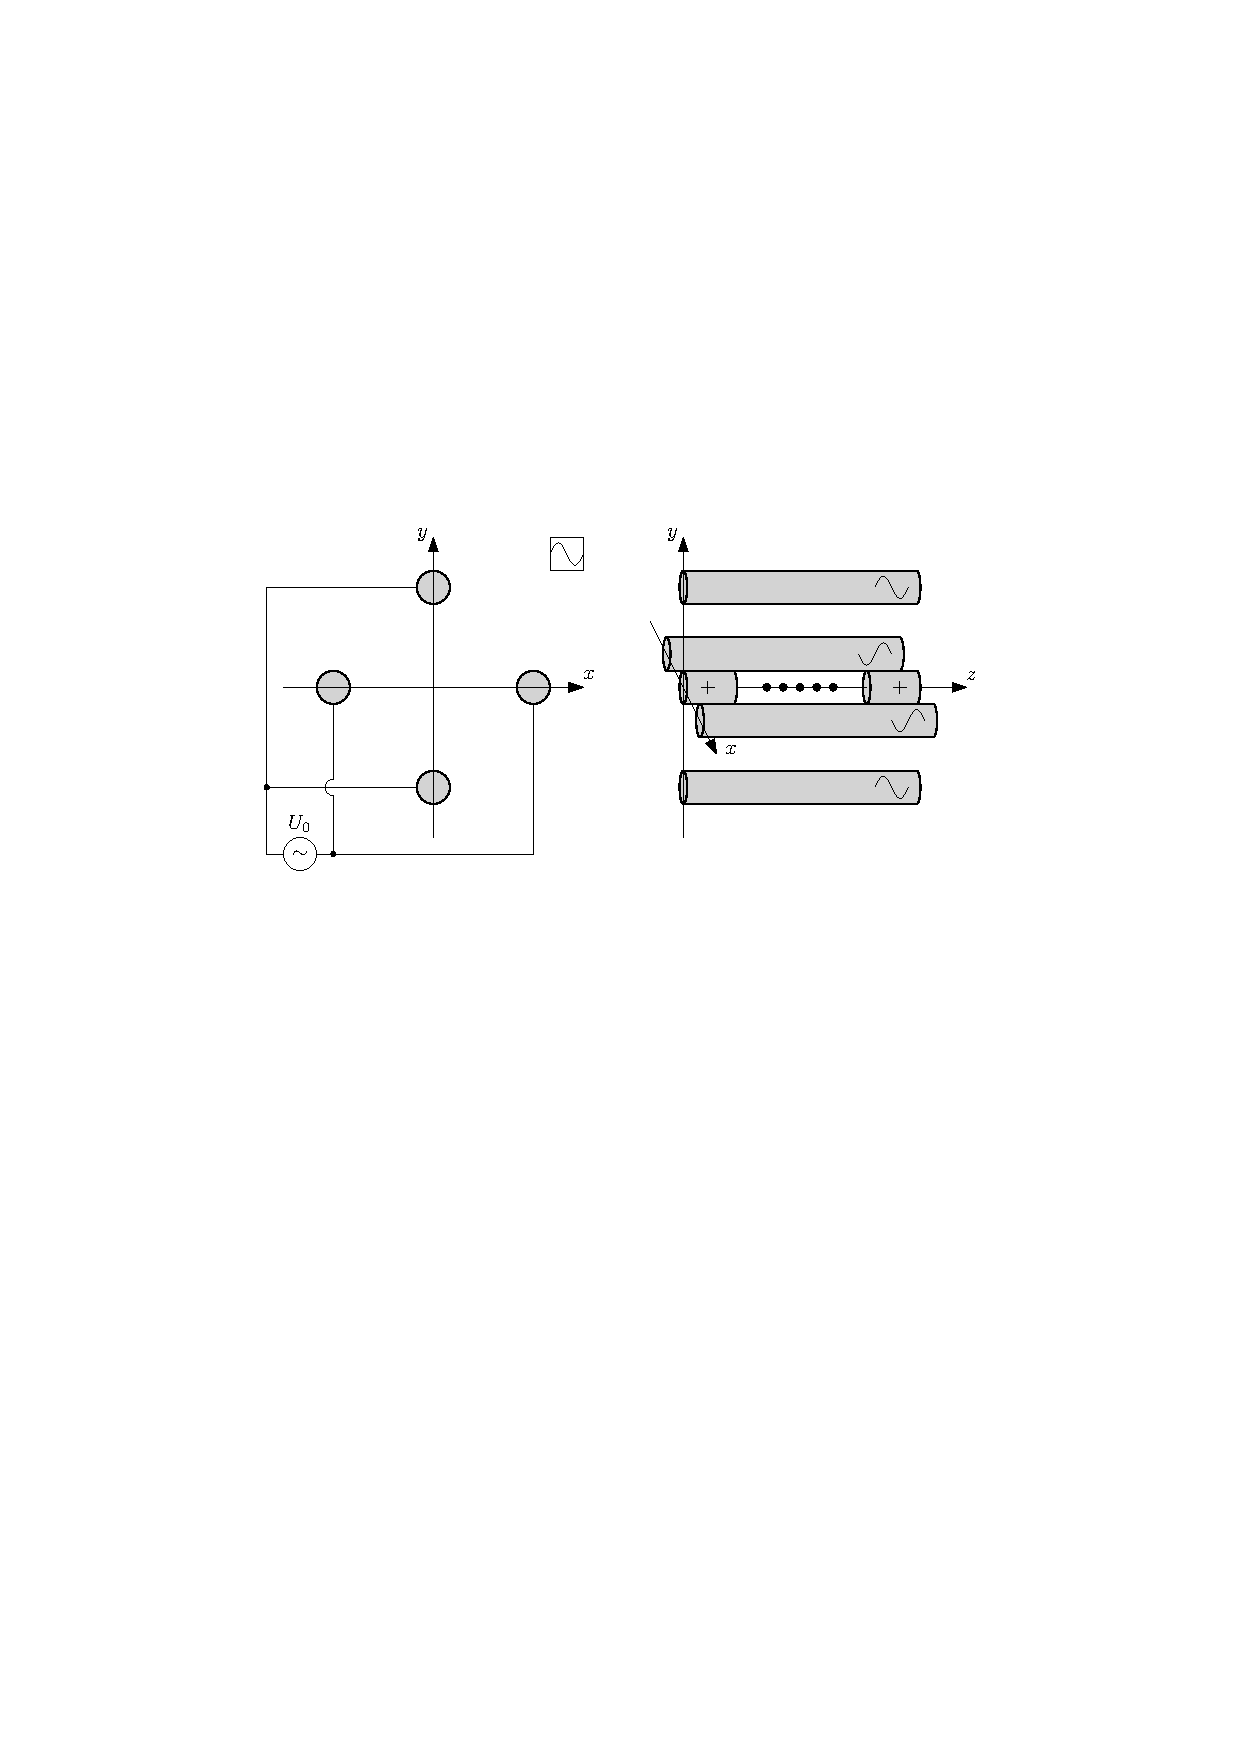
\includegraphics[width=1\textwidth]{./figures/lineare_paulfalle.pdf}
			\end{figure}
	\end{columns}
	
	\vspace{0.2cm}
		
	\begin{figure}[h]
		\centering
		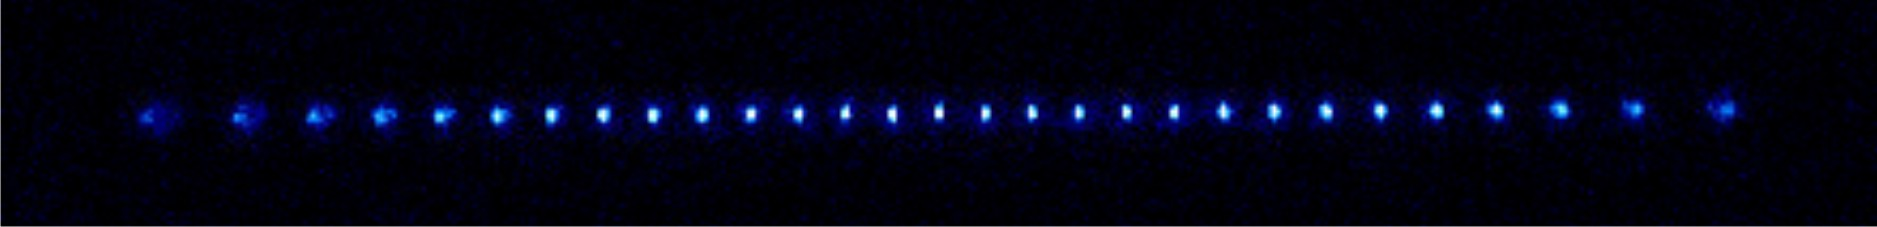
\includegraphics[width=0.8\textwidth]{./figures/29_laser_cooled_ion_chain.jpg}
		\caption{Lasergekühlte Thorium-Atome ($\mathrm{Th}^{3+}$) in einer linearen Paul-Falle (Abstand etwa \SI{50}{\micro\metre}) \cite{campbell}}
	\end{figure}
	
\end{frame}

%\begin{frame}{Lineare Paul-Falle}
%Axiale Kraft kleiner als Radiale:
%\begin{figure}[h]
%	\centering
%	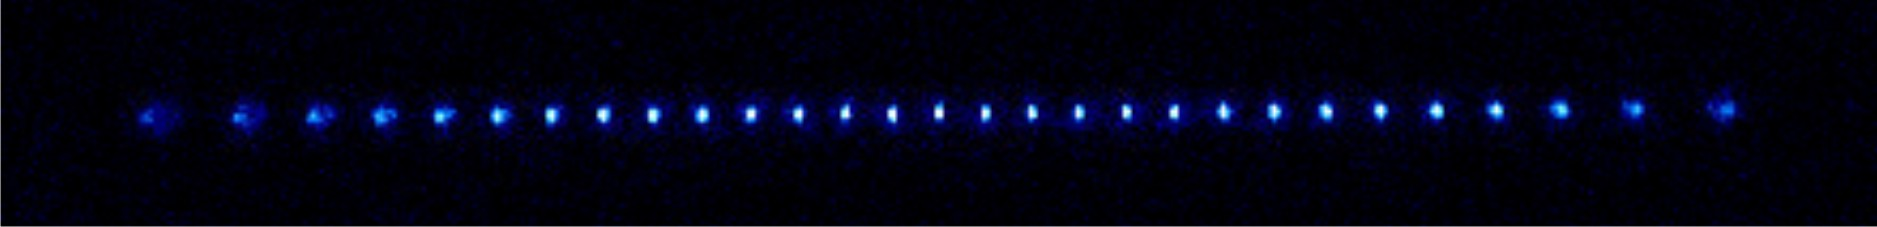
\includegraphics[width=0.9\textwidth]{./figures/29_laser_cooled_ion_chain.jpg}
%	\caption{29 lasergekühlte Thorium-Atome ($\mathrm{Th}^{3+}$) in einer linearen Paul-Falle (Abstand etwa \SI{50}{\micro\metre}) \cite{campbell}}
%\end{figure}
%
%(Penning-Falle?)
%
%\end{frame}

\section{Magneto-optische Falle}

\begin{frame}{Streukraft}
	\begin{columns}[t]
		\column{0.5\textwidth}
		\begin{itemize}
			\item Photonenimpuls:
			\begin{align*}
				p = \frac{E}{c}
			\end{align*}
			\item Impulsübertrag durch Absorption
			
			\item isotrope Emission
			
			\item[$\Rightarrow$] im statistischen Mittel: Kraft in Laserrichtung
		\end{itemize}
		
		\column{0.5\textwidth}
		\begin{figure}[h]
			\centering
			\vspace{-1cm}
			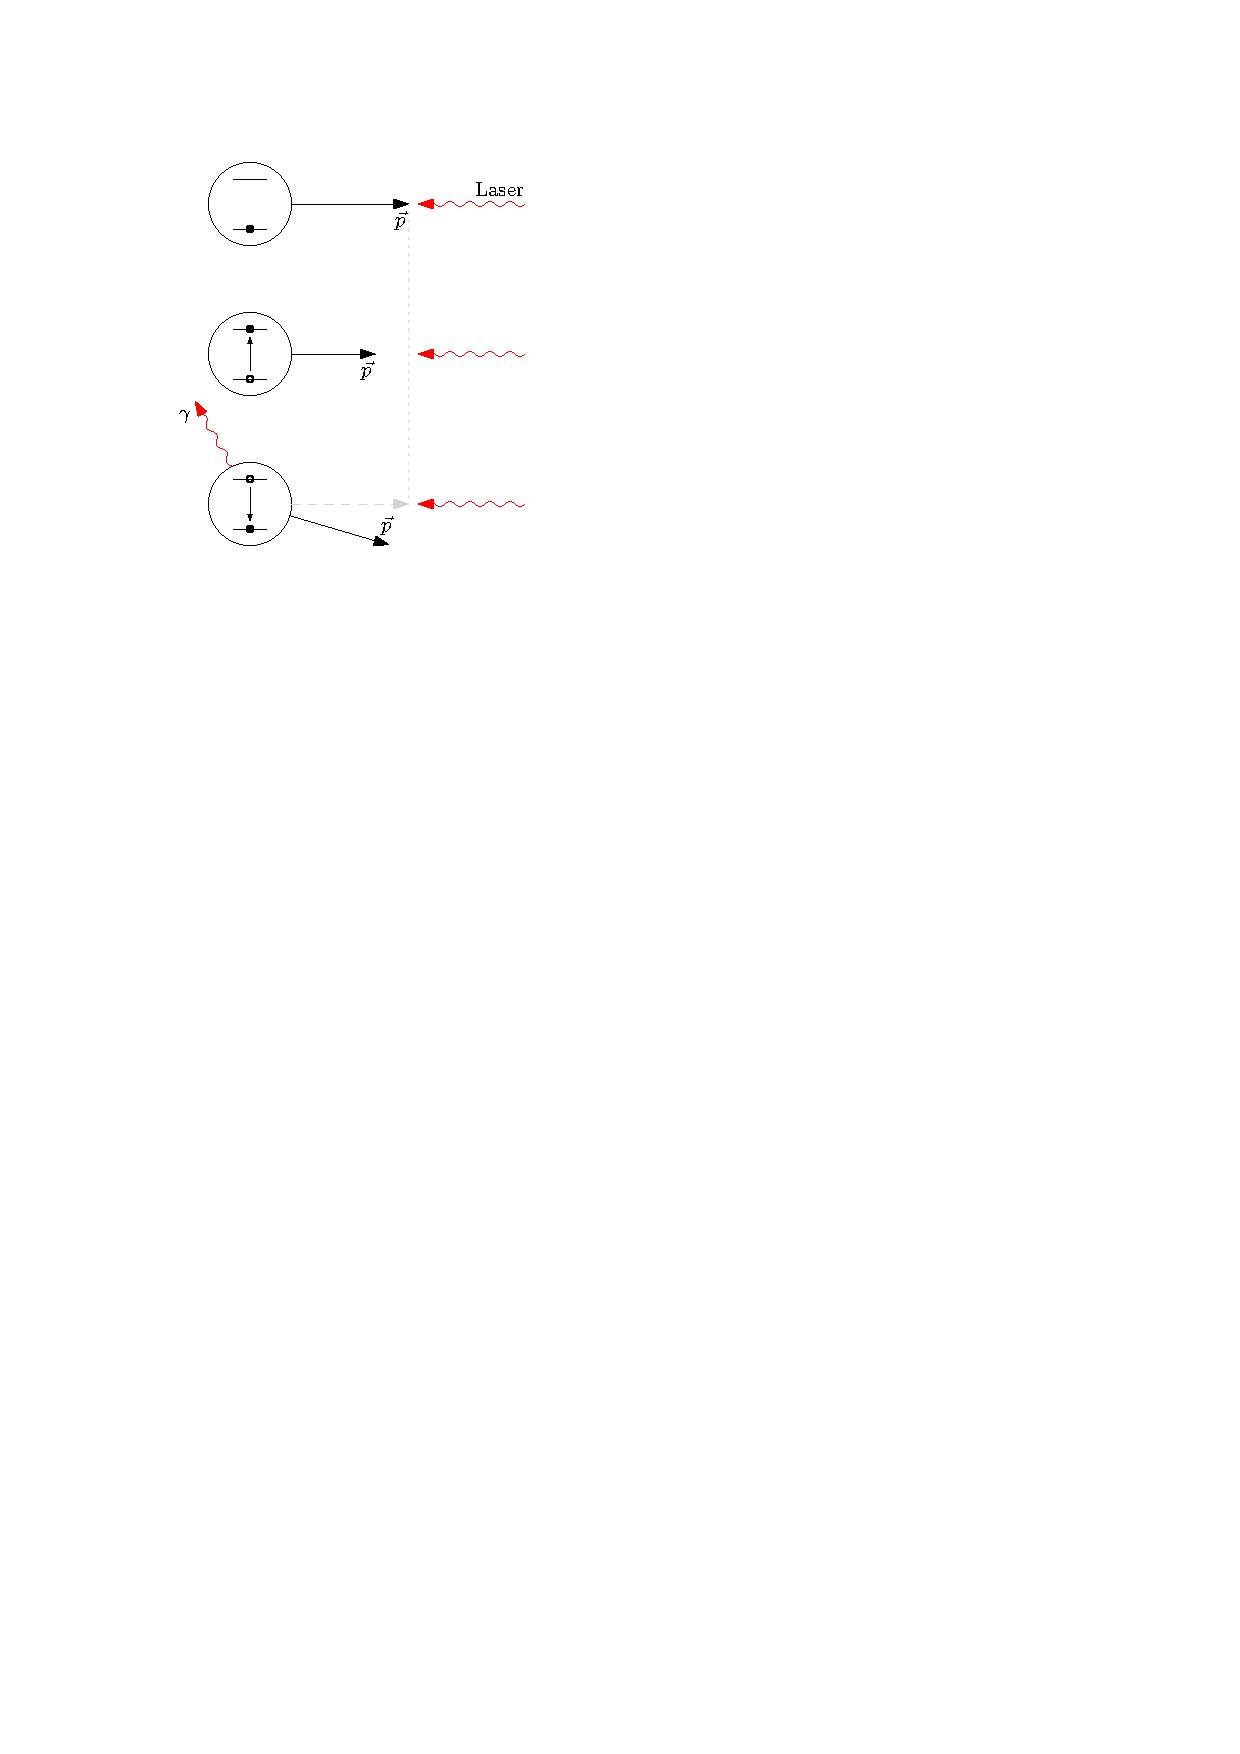
\includegraphics[width=1.0\textwidth]{./figures/streukraft.pdf}
		\end{figure}
		
	\end{columns}

\end{frame}

\begin{frame}{Magneto-optische Falle}
\begin{itemize}
	\item Zeeman-Effekt: $\Delta E = g_J \mu_\mathrm{B} m_J B$ \korr{Magnetfeld klarmachen}
\end{itemize}

\vspace{0.5cm}

\begin{figure}[h]
	\centering
	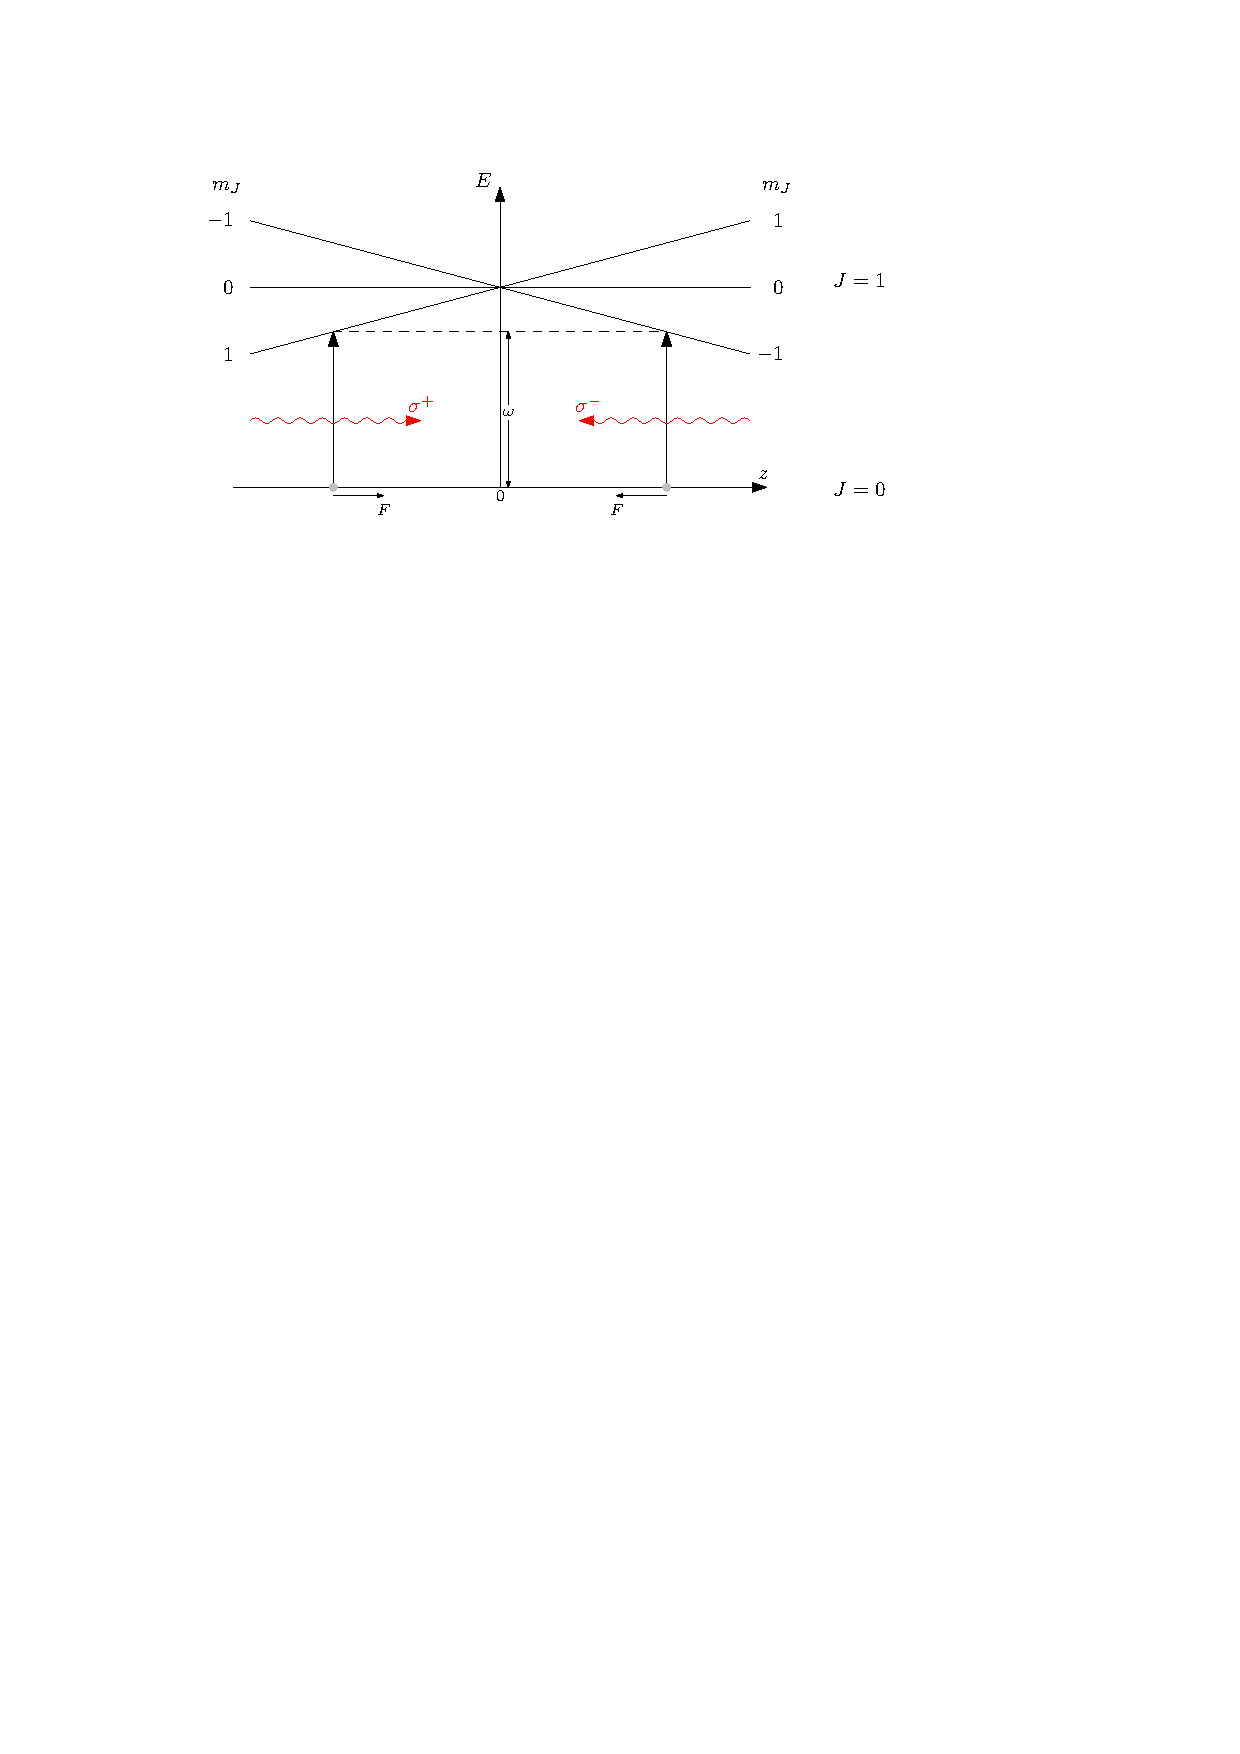
\includegraphics[width=1\textwidth]{./figures/mot.pdf}
\end{figure}
\end{frame}

\begin{frame}{Magneto-optische Falle}
\begin{columns}
\column{0.5\textwidth}
\begin{itemize}

	\item Magnetfeldgradient durch Anti-Helmholtzspulenpaar
		
	\item drei Paare gegenläufiger Laser entsprechender Polarisation

\end{itemize}

\column{0.5\textwidth}
	\begin{figure}
		\centering
		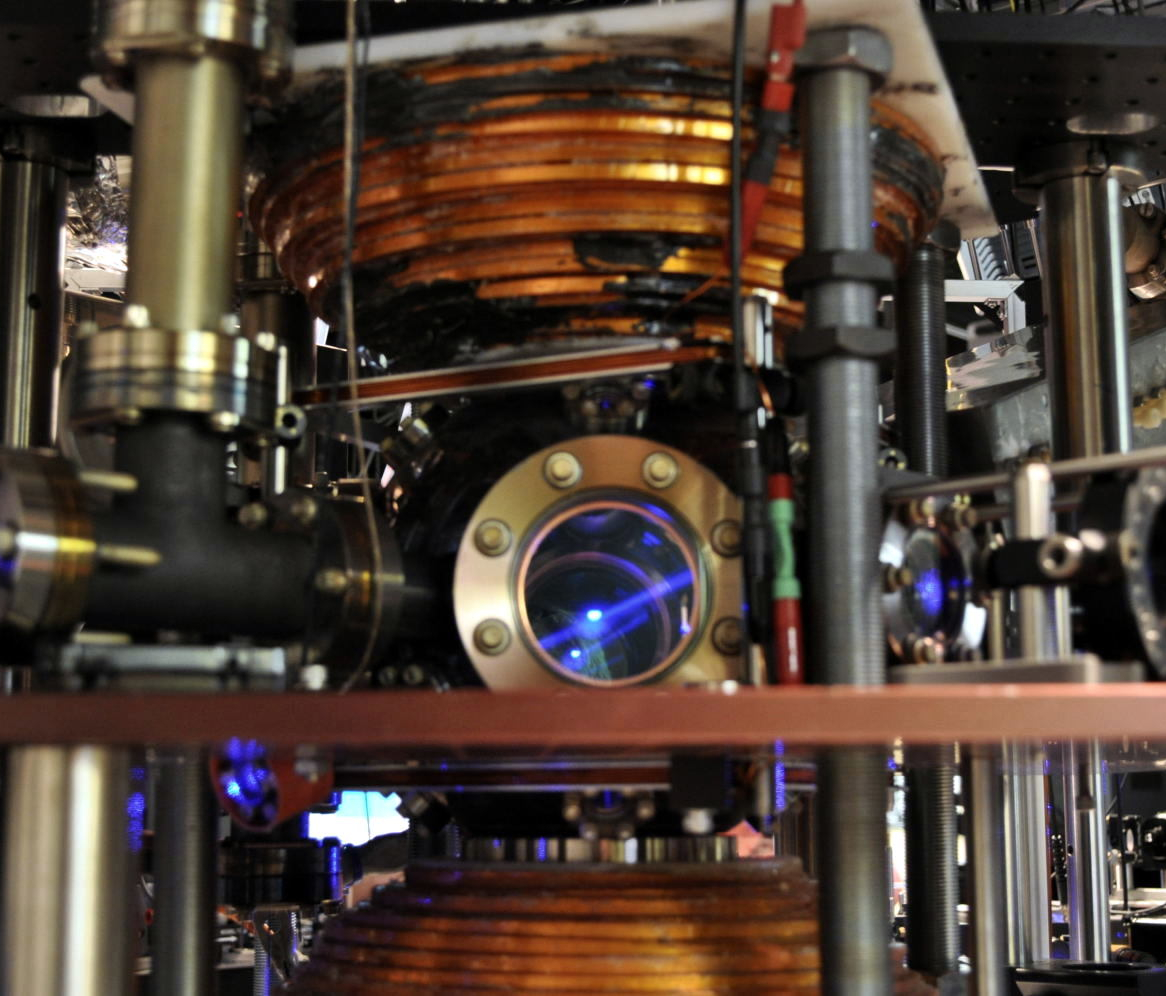
\includegraphics[width=0.9\textwidth]{./figures/mot_columbia.jpg}
		\caption{Magneto-optische Falle \cite{columbia}}
	\end{figure}
\end{columns}
\end{frame}


\section{Magnetfalle}

\begin{frame}{Magnetfalle}
	\begin{columns}
	\column{0.5\textwidth}
	\begin{itemize}
		\item Zeeman-Energie des Atoms im Zustand $\ket{I J F m_F}$:
		\begin{align*}
			E = g_F \mu_\mathrm{B} m_F B
		\end{align*}
		
		\item \textcolor{red}{Schwachfeldsucher:} $g_F m_F > 0$
		
		\item \textcolor{blue}{Starkfeldsucher:} \\$g_F m_F < 0$
		
		\item Min. oder Max. von $|\vec{B}|$ benötigt um Atom zu fangen
		
		\item kein Maximum möglich, da $\divergence \vec{B} = 0$
	\end{itemize}
	\column{0.5\textwidth}
		\begin{figure}
			\centering
			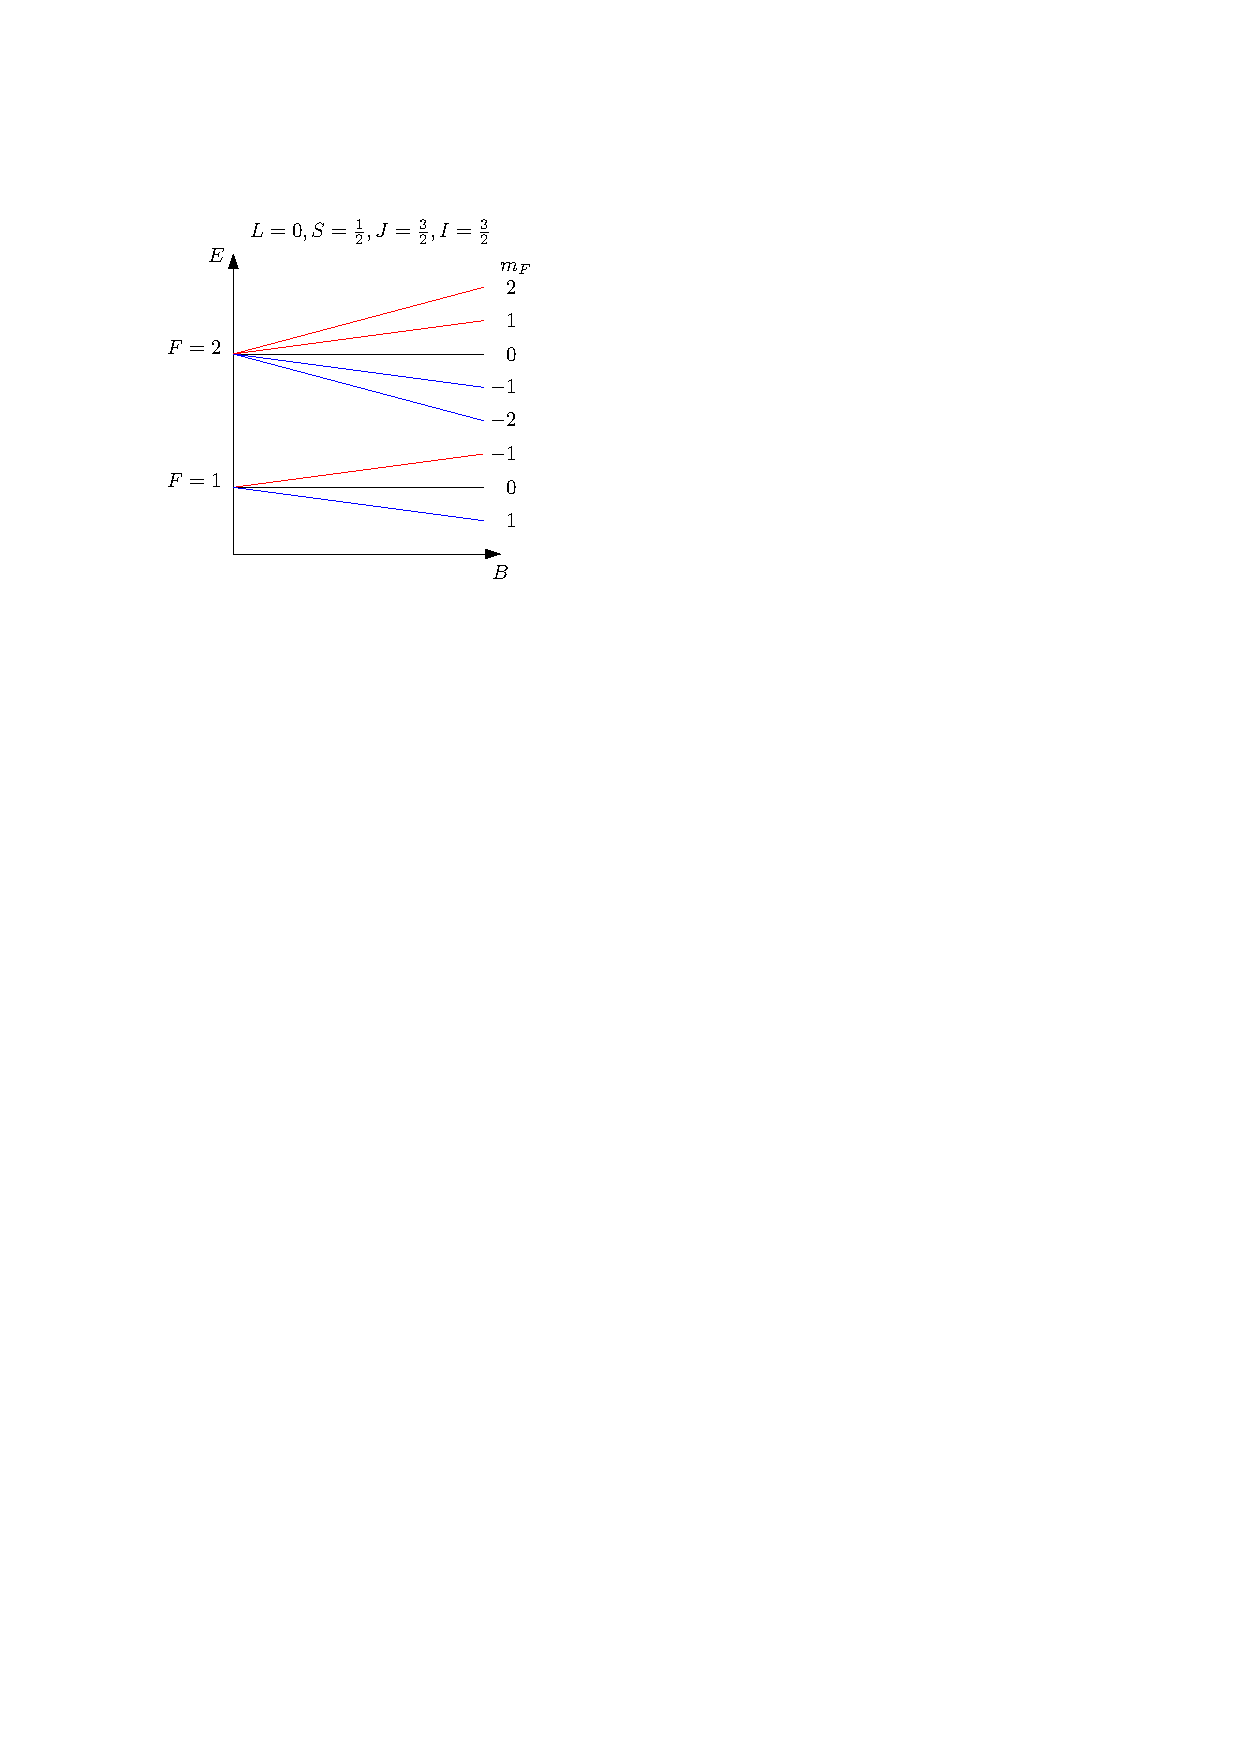
\includegraphics{./figures/magnetfalle.pdf}
		\end{figure}
	\end{columns}
\end{frame}


\section{Vergleich der Fallen}

\begin{frame}{Vergleich der Fallen}
	
	\resizebox{\textwidth}{!}{
	{\def\arraystretch{1.5}\tabcolsep=5pt
	\begin{tabular}{l | p{4cm} | p{4cm} | p{4cm} }
		& Paul-Falle & Magneto-optische Falle & Magnetfalle \\
		\hline
		typ. Fallentiefen: & $\sim \SI{1e6}{K}$ & $\sim \SI{1}{K}$ & $\sim \SI{10}{mK}$\\
		min. Temperatur: & $\sim \SI{1}{mK}$ & $\sim \SI{100}{\micro\kelvin}$ & $\sim \SI{10}{nK}$ \\
		&&&\\
		Vor- / Nachteile: & \textcolor{Red}{nur Ionen} & \textcolor{Green}{neutrale Atome} & \textcolor{Green}{neutrale Atome}\\
		& \textcolor{Green}{zustandsunabhängig} & \textcolor{Red}{zustandsabhängig} & \textcolor{Red}{zustandsabhängig}\\
		& & \textcolor{Green}{Kühlung durch Melasse} &\textcolor{Green}{keine untere Grenze}\\
		& \textcolor{Green}{Ionisation direkt in der Falle} & \textcolor{Green}{Einfangen von Atomen bei Raumtemperatur} & \textcolor{Red}{vorangehende Kühlstufe benötigt} \\
	\end{tabular}}}
	
\end{frame}

\begin{frame}{Vielen Dank für die Aufmerksamkeit}
\end{frame}

\section{Literatur}

\begin{frame}{Literatur}
	\begin{thebibliography}{9}
		\bibitem{foot}
		Christopher J. Foot,
		\emph{Atomic Physics},
		Oxford University Press 2005
		
		\bibitem{campbell}
		Corey J. Campbell,
		\emph{Trapping, Laser Cooling, and Spectroscopy of Thorium IV},
		Georgia Institute of Technlogy 2011
		
		\bibitem{wpw}
		Carl E. Wieman, David E. Pritchard, David J. Wineland,
		\emph{Atom cooling, trapping, and quantum manipulation},
		Reviews of Modern Physics, Vol. 71, No.2 1999
		
		\bibitem{columbia}
		Columbia University: Department of Physics,
		\url{http://physics.columbia.edu/research/atomic-molecular-optical-physics},
		(Letzter Aufruf 22. Mai 2015)
		
		
	\end{thebibliography}
	
\end{frame}

\begin{frame}{Anhang}
	\begin{figure}
		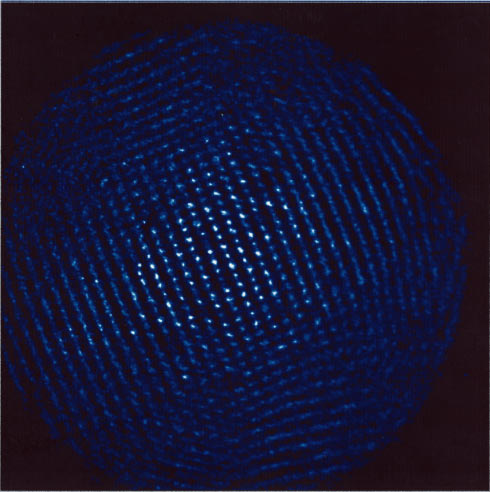
\includegraphics[width=0.5\textwidth]{./figures/ionenkristall.png}
		\caption{Ionenkristall aus lasergekühlten Berylliumatomen in einer Penning-Falle \cite{wpw}}
	\end{figure}
\end{frame}

\begin{frame}{Optische Melasse}
\begin{figure}[h]
	\centering
	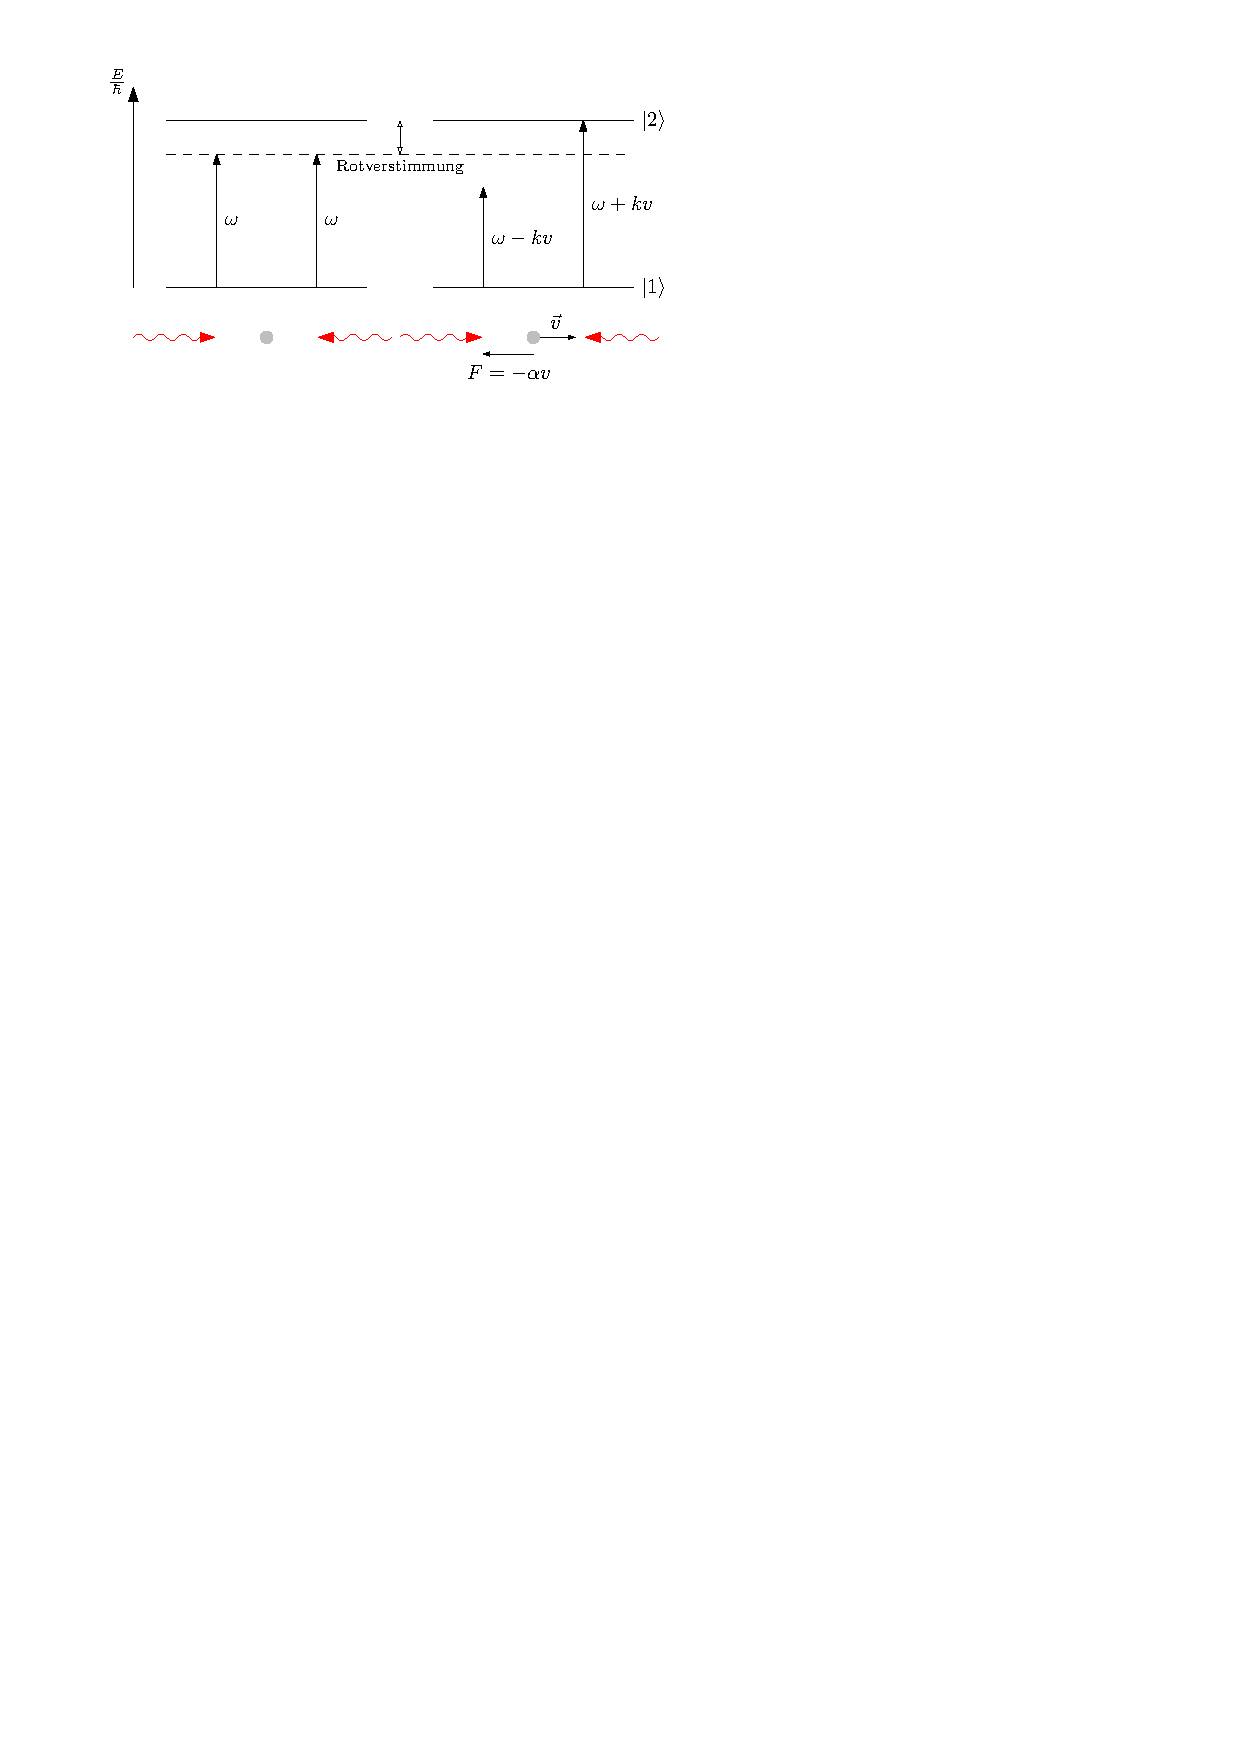
\includegraphics[width=\textwidth]{./figures/melasse.pdf}
\end{figure}
\end{frame}

\end{document}